\documentclass[a4paper,12pt]{article}

\usepackage[utf8]{inputenc}
\usepackage[T1]{fontenc}
\usepackage{a4}
\usepackage{lipsum}
\usepackage{graphicx}
\usepackage{float}
\usepackage{listings}
\usepackage{color}
\usepackage{hyperref}
\usepackage{cite}
\usepackage{textgreek}
\usepackage{amsfonts}

\usepackage[margin=1in]{geometry}

\definecolor{dkgreen}{rgb}{0,0.6,0}
\definecolor{gray}{rgb}{0.5,0.5,0.5}
\definecolor{mauve}{rgb}{0.58,0,0.82}

\lstset{frame=tb,
  language=matlab,
  aboveskip=5mm,
  belowskip=5mm,
  showstringspaces=false,
  columns=flexible,
  basicstyle={\small\ttfamily},
  numberstyle=\tiny\color{gray},
  keywordstyle=\color{blue},
  commentstyle=\color{dkgreen},
  stringstyle=\color{mauve},
  breaklines=true,
  breakatwhitespace=true,
  tabsize=2
}

\title{
  {\Huge \bf Power Systems Lab}\\
  \vspace{0.25in}

  {\bf Experiment 6}\\
  Laboratory Report
  \vspace{1in}
}
\author{
  \bf Syed Alisamar Husain, 17BEE012\\
  B.Tech Electrical Engg, 8th Semester
}

\begin{document}
  \begin{titlepage}
    \maketitle
    \vspace*{\fill}
    \begin{center}
      {\bfseries Department of Electrical Engineering} \\
      Jamia Millia Islamia, New Delhi
    \end{center}
    \thispagestyle{empty}
  \end{titlepage}
  
  \newpage
  \begin{center}
    \huge Experiment 6
    \vspace{0.5in}
  \end{center}

  \section{Objective}
  Study and describe the various elements in the SimPowerSystems library of Simulink.

  \section{Background}
    \subsection{About the Library}
    Simscape Electrical (formerly SimPowerSystems) 
    provides component libraries for modeling and simulating electronic, 
    mechatronic, and electrical power systems. It includes models of 
    semiconductors, motors, and components for applications such as 
    electromechanical actuation, smart grids, and renewable energy systems. 
    
    These components can be used to evaluate analog circuit architectures, 
    develop mechatronic systems with electric drives, and analyze the generation, 
    conversion, transmission, and consumption of electrical power at the grid level.

    The SimPowerSystems library contains more than 150 blocks distributed in 
    sublibraries such as:
    \begin{itemize}
      \item {\bf Electrical sources}: voltage and current sources
      \item {\bf Circuit elements}: transformers, RLC branches, loads, transmission lines, etc.
      \item {\bf Machinery}: AC and DC motors, generators, turbines and governors
      \item {\bf Power electronics}: power switches (diodes, thyristors, GTOs, IGBTs, etc.)
      \item {\bf Measurement}: voltage, current and impedance measurement instruments
    \end{itemize}

    SimPowerSystems’ open architecture allows models to be adapted to specific
    needs. This flexibility, combined with the wide variety of easy-to-use blocks, makes
    SimPowerSystems the ideal prototyping platform for studying new power system
    models and for understanding complex control systems.
   
    \subsection{Usage}
    Simscape Electrical helps to develop control systems and test system-level 
    performance. One can parameterize your models using MATLAB variables and 
    expressions, and design control systems for electrical systems in Simulink. 
    One can integrate mechanical, hydraulic, thermal, and other physical systems 
    into the model using components from the Simscape family of products. 
    To deploy models to other simulation environments, including 
    hardware-in-the-loop (HIL) systems, Simscape Electrical supports C-code 
    generation.

  \begin{figure}[H]
    \centering
    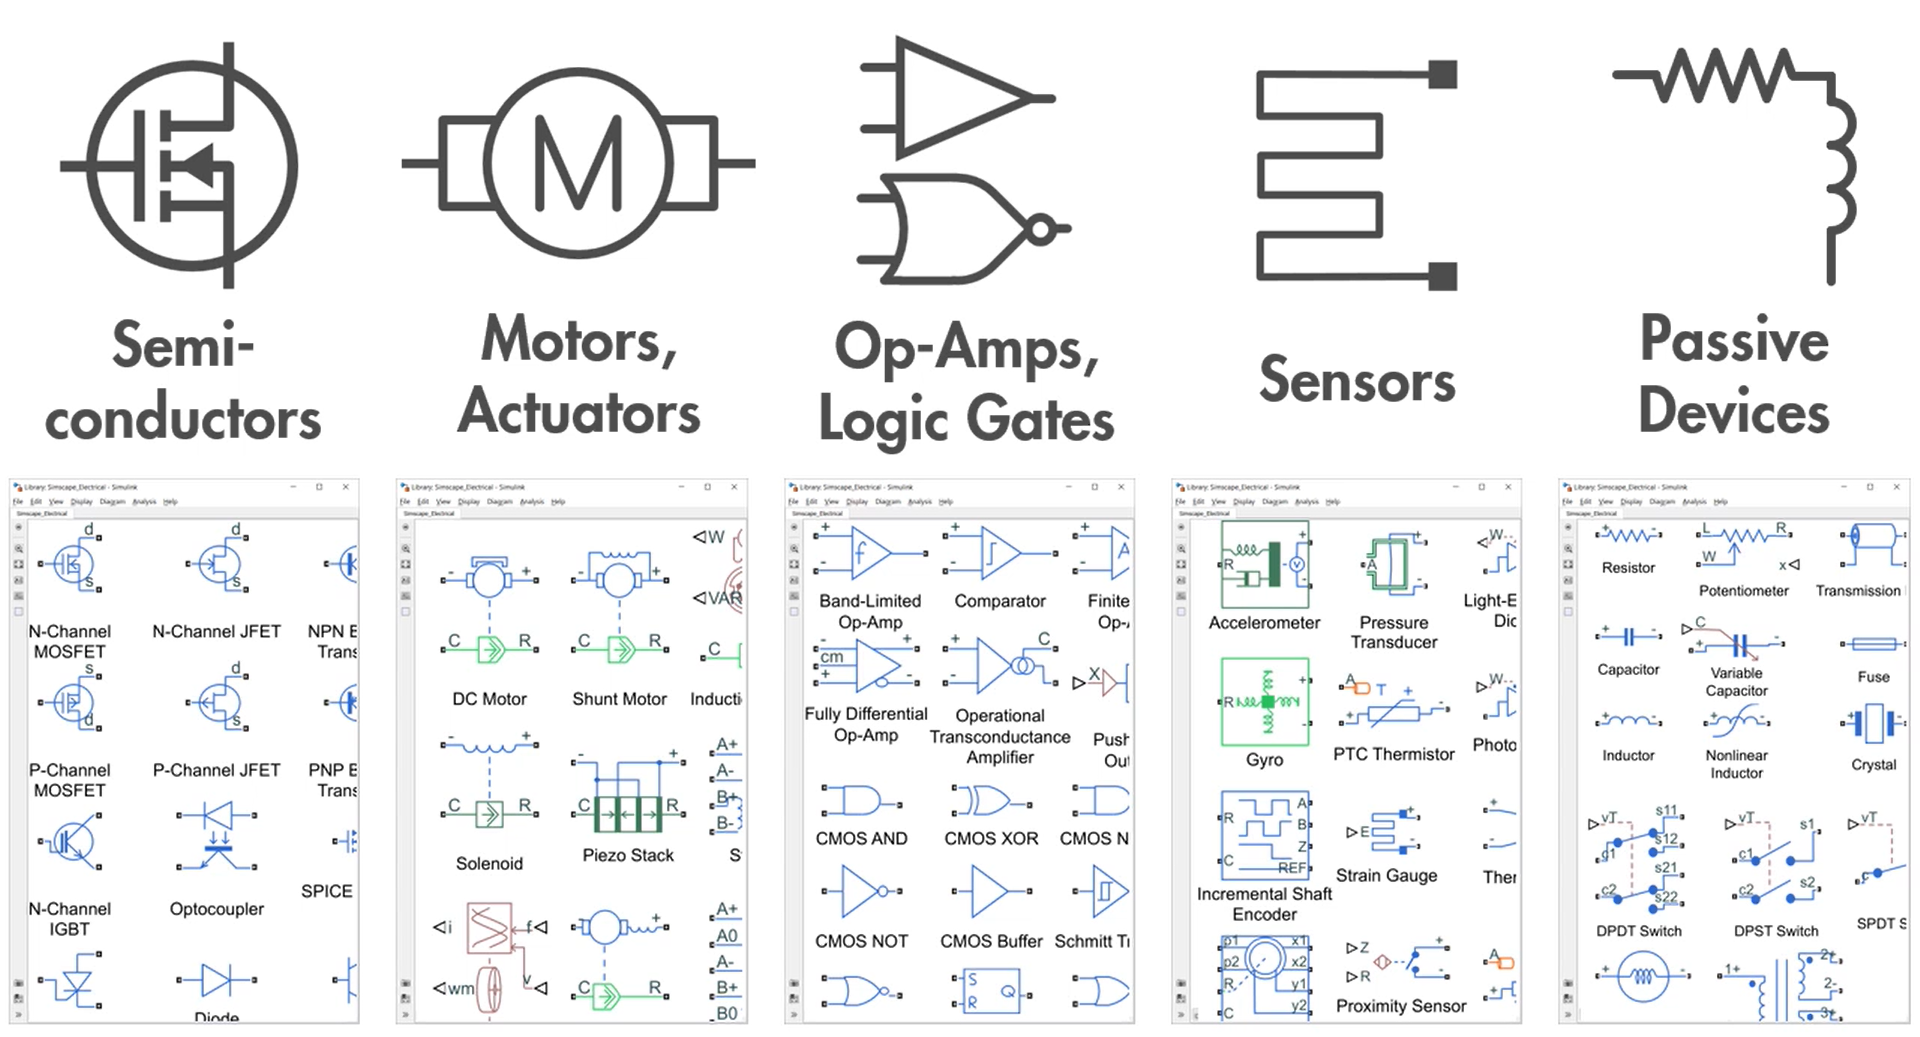
\includegraphics[width=3in]{img/Screenshot (37).png}
    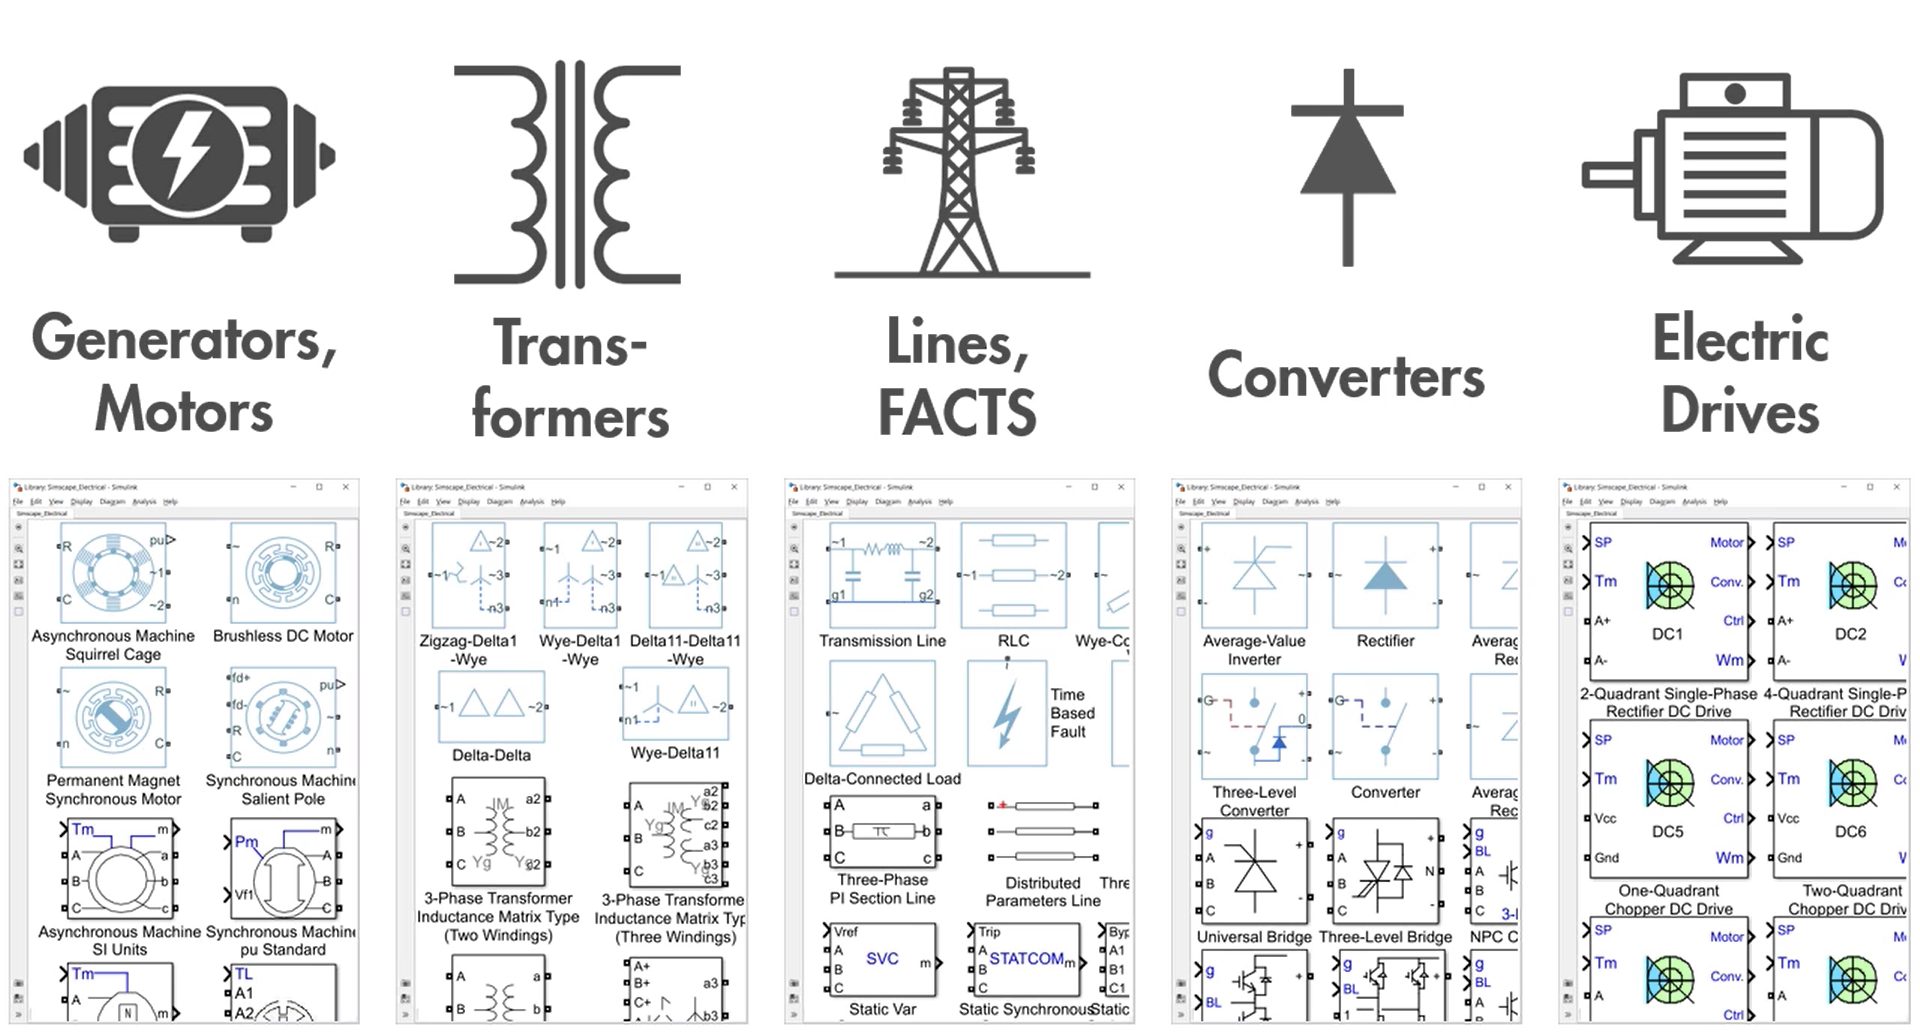
\includegraphics[width=3in]{img/Screenshot (38).png}
  \end{figure}

  \section{Simscape Electrical}
    \subsection{Block Libraries}
    Simscape Electrical libraries include {\bf blocks} and models of semiconductors, 
    motors, and components for applications such as electromechanical actuation, 
    smart grids, and renewable energy systems. You can use these component 
    libraries for modeling and simulating electronic, mechatronic, and electrical 
    power systems. 

    These are also used to evaluate analog circuit architectures,​ develop mechatronic 
    systems with electric drives,​ and analyze the generation,​ conversion,​ 
    transmission,​ and consumption of electrical power at the grid level.

    \subsection{Some Elements in the Libraries}
    {\bf Connectors and References​}
    \begin{itemize}
      \item Busbar: Load flow analysis busbar connector
      \item Delta Reference (3$\phi$): Internal reference point for delta-connected network
      \item Floating Neutral (3$\phi$): Internal floating neutral point for wye-connected network
      \item Grounded Neutral (3$\phi$): Connect phases of three-phase system to reference
      \item Neutral Port (3$\phi$): Connect phases of three-phase system to neutral
      \item Open Circuit (3$\phi$): Three-phase terminator that draws no current
      \item Phase Permute: Permute phases of three-phase system
      \item Phase Splitter: Expand or combine three electrical conserving ports
    \end{itemize}
    {\bf Integrated Circuits (General Circuits​)}
    \begin{itemize}
      \item Band-Limited Op-Amp	Model
      \item Comparator: Behavioral model of a comparator integrated circuit
      \item Controlled PWM Voltage: Pulse-width modulated voltage source
      \item Finite-Gain Op-Amp: Gain-limited operational amplifier model with optional noise
      \item Fully Differential Op-Amp: Operational amplifier with fully differential output, that is, not referenced to ground
      \item Multiplier: Integrated circuit multiplier
      \item Timer: Behavioral model of a timer integrated circuit
      \item Voltage-Controlled Oscillator: Behavioral model of voltage-controlled oscillator
    \end{itemize}
    {\bf Switches and Breakers}
    \begin{itemize}
      \item Circuit Breaker	Single-pole single-throw circuit breaker
      \item Circuit Breaker (Three Phase)	Three-phase circuit breaker controlled by external signal
      \item Circuit Breaker (with arc)	Single-pole single-throw circuit breaker with Mayr arc representation
      \item DPDT Switch	Double-pole double-throw switch
      \item Fuse	Fuse that protects against excessive current
    \end{itemize}
    {\bf Relays}
    \begin{itemize}
      \item SPDT Relay: Single-pole, double-throw relay with delays and faults
      \item SPST Relay: Single-pole single-throw relay with delays and faults
    \end{itemize}
    {\bf Lines}
    \begin{itemize}
      \item PI Section Line: transmission line with lumped parameters
      \item Distributed Parameters Line: N-phase distributed parameter transmission line model with lumped losses
      \item Three-Phase PI Section Line: three-phase transmission line section with lumped parameters
    \end{itemize}

  \section{Result}
  We studied and described a few block elements from the libraries in SimPowerSystems
  application of SIMULINK, now known as Simscape Electrical.

\end{document}